\documentclass[12pt]{article}

\usepackage[paper=a4paper,left=25mm,right=25mm,top=25mm,bottom=25mm]{geometry}
\usepackage{url}
\usepackage{notoccite}
\usepackage{graphicx}
\usepackage{multirow}
\graphicspath{ {images/} }

\title{Projeto SMA, Rock Paper Scissors Lizard Spock}
\author{José Ferreira (53311), Afonso Seguro (57700)}

\begin{document}
	
	\maketitle
	
	\section*{Introdução}
	
	\newpage
	\section*{Contexto}
	O projeto que foi decidido implementar foi o “rock paper scissors lizard spock”, uma variação do jogo tradicional, “pedra papel tesoura”, que implementa mais 2 novas personagens (lizard, spock).\\
    Este jogo consiste num número mínimo de 2 jogadores que podem escolher apenas uma das personagens intervenientes para jogar, obtendo uma cotação quando defrontado, positiva (1) caso ganhe, negativa (-1) caso perca. Isto é repetido na sucessão de 15 rondas, sendo que cada jogador obtém 3 vezes cada umas das personagens iniciais, indo gastando-as a medida do decorrer das rondas.\\
    Para ser implantado numas plataformas para sistemas de vários agentes, como o Jade, este jogo tem de conter um agente interveniente que vai regular todas as rondas, a medida que o jogo avança. Este mesmo agente chama-se mestre, pois é dele que todo o jogo vai depender.\\
    Todos os agentes são deliberativos, ou seja, todas as suas jogadas são fundamentadas em função daquilo que sabem, dos seus desejos e das suas intenções, tendo cada agente jogador uma maneira diferente para implementar vários planos em prol de alcançar o máximo de pontos possíveis.\\
    Para os jogadores, foi decidido implementar 5 tipos diferentes de agentes, tendo cada um deles um algoritmo diferente para gerar planos de modo a cumprir desejos e intenções.\\
    
    Estes são:

    \begin{itemize}
        \item Jogador Minor
        \item Jogador MinMax
        \item Jogado Prob
        \item Jogador All 1
        \item Jogador All 2
        \item Jogador Dummy
    \end{itemize}

    
    Iremos fazer uma breve explicação deles na arquitetura de cada agente mais a frente.
	
	\newpage
	\section*{Arquitetura Geral}
	Como já referido no contexto, este jogo consiste na criação de vários agentes jogadores que são regidos por um agente mestre.\\
    O agente mestre, é peça central de todo o jogo, mas, no entanto, não necessita de ser tão deliberativo como os agentes jogadores, pois apenas tem de recolher e calcular todas as jogadas de todos os intervenientes. Para tal, a maneira de como ele alcança todos os outros, é deveras importante para o bom funcionamento do jogo. \\
    Para este problema, foi escolhida uma abordagem inicial de utilizar o “Contract Network Protocol”, no entanto, tendo a necessidade de utilizar vários behaviours , a utilização de uma função apenas para responder com a jogada ao mestre, tornar complicada a implementação de uma arquitetura deliberativa. Isto demonstrado nas classes Mestre CN e Jogador CN.\\
    A solução escolhida, a criação do próprio protocolo de comunicação, este tem um funcionamento muito simples, pois apenas envia as jogadas antigas aos jogadores, espera que todos respondam, e faz o cálculo dos pontos consoante as jogadas, isto repetidamente durante 15 rondas.
    
    	
	\begin{figure}[h]
		\centering
		\includegraphics[width=0.65\textwidth]{arquiteturageral.eps}
		\caption{Arquitetura Geral}
		\label{fig:arquiteturageral}
	\end{figure}
	
	
	Na primeira ronda como não há jogadas anteriores, é enviado o índex do jogador, ou seja, no array onde são enviadas as jogadas anteriores, qual a iteração que mostras as suas jogadas.\\
	
	
	\newpage
	\section*{Arquitetura interna dos agentes}
	
	Nesta secção vamos mostrar a arquitetura interna dos agentes, quais os behaviors que os constituem, onde e como são calculados os planos consoante as crenças, os desejos e as intenções, e como tudo junto resulta na ação.\\
	
    Como já interpelado, vamos abordar estes agentes:\\

    \begin{itemize}
        \item Jogador Mestre
        \item Jogador Minor
        \item Jogador MinMax
        \item Jogado Prob
        \item Jogador All 1
        \item Jogador All 2
        \item Jogador Dummy
    \end{itemize}
	
	
	\subsection*{Mestre}
	O mestre, como já referido, não é propriamente um agente deliberativo, pois não cria planos nem os altera consoante intenções ou desejos, no entanto também não é um agente reativo, pois as suas ações são previamente calculadas, guardando jogadas e calculando classificações.\\
    Este mesmo é constituído por 4 behaviour, como mostrada na figura abaixo, sendo o Play Behavior o mais importante. Todos os outros são auxiliares ao bom funcionamento do jogo, como a recolha de agentes (Ticket Behaviour) ou a capacidade de repetir vários jogos (Cyclic Behaviour).\\
    
    \begin{figure}[h]
		\centering
        \includegraphics[width=0.80\textwidth]{mestre.eps}
		\caption{Behaviours mestre}
		\label{fig:mestre}
	\end{figure}
	
	O Play Behavior é a alma do jogo, pois é este comportamento que permite o desenrolar de um jogo, como demonstrado no algoritmo abaixo, este behaviour começa por enviar as jogadas 
    anteriores, à exceção da primeira, que envia o index do jogador, para o mesmo saber quais as suas jogadas, depois fica a espera de todas as respostas, quando chega, calcula as classificações, e se chegar as 15 rondas, mostras as classificações.\\

	\begin{figure}[h]
		\centering
        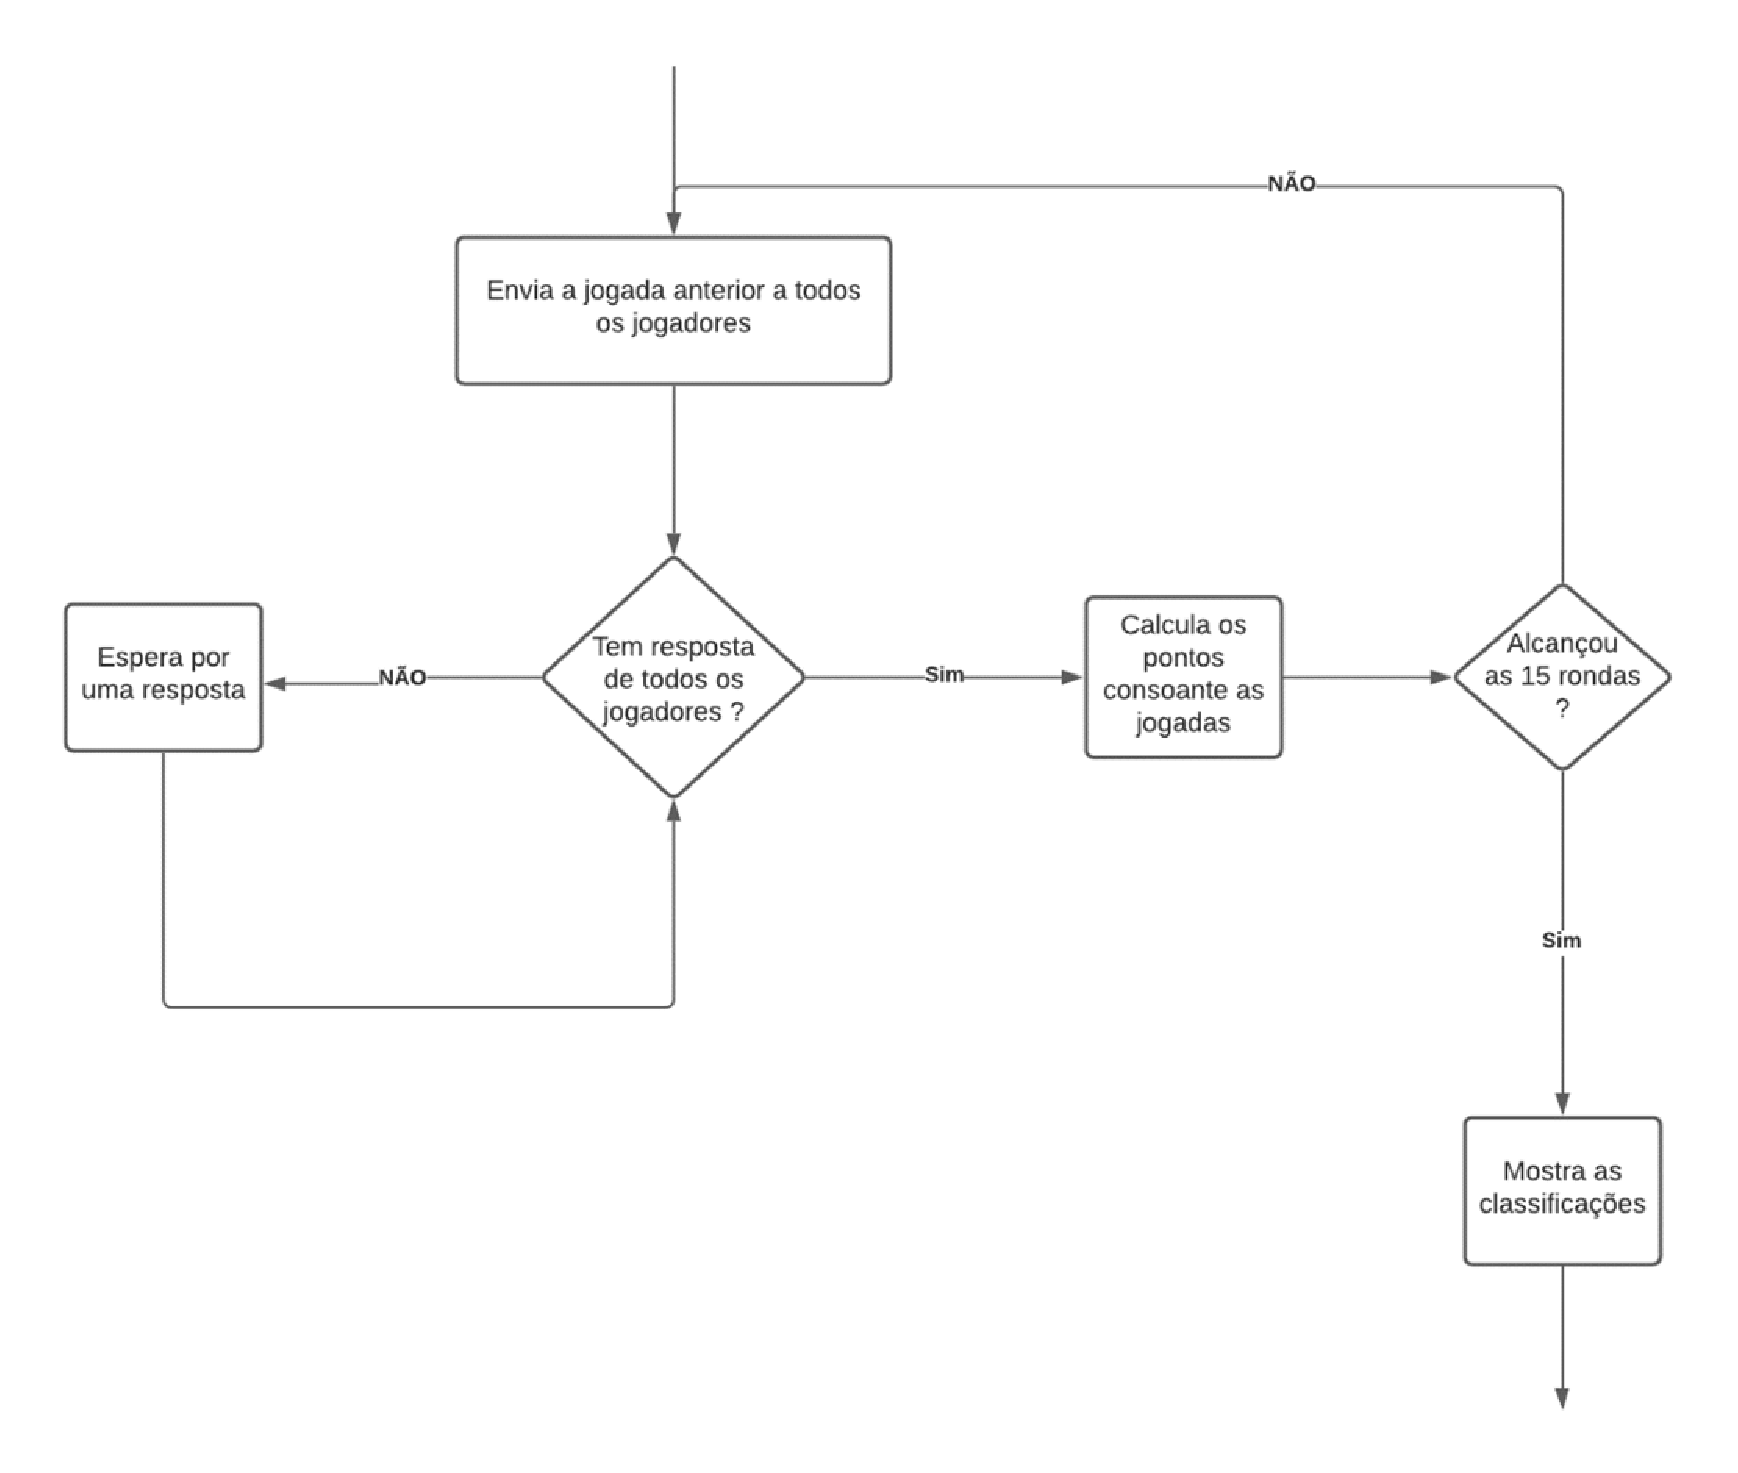
\includegraphics[width=0.80\textwidth]{mestrealg.eps}
		\caption{Play Behaviour mestre}
		\label{fig:mestrealg}
	\end{figure}
	

    Para acionar o mestre a começar um jogo, um agente Dummy, tem de enviar uma mensagem do tipo REQUEST, essa mensagem vai fazer o mestre lançar um Play Behaviour e assim começar um jogo com os agentes que conhece\\
	
	\subsection*{Jogador}
	Os jogadores em si, têm todos uma arquitetura idêntica, á exceção do dummy, isto porque a base é igual visto que todos funcionam com um assento em três pilares:\\
	
	
	\begin{itemize}
        \item Crenças - Onde o jogador, recolhe todos os dados que sabe sobre o ambiente, ou seja, quais as mãos que lhe sobram, quais as mãos que sobram aos outros jogadores, quantas rondas faltam, etc…
        
        \item Desejos - O agente calcula quais as jogadas, ou sequência de jogadas, que pode realizar, ou seja, vários planos.
        
        \item Intenções - Este escolhe dos vários planos apresentados, quais os melhores, em prol do objetivo final de obter mais pontos.
    \end{itemize}

    
    A figura abaixo indica como é realizada a arquitetura base de cada agente jogador, consiste em 4 behaviours.\\
    O cyclic behaviour, apenas espera que por mensagens do mestre, e envia as jogadas realizadas para outros agentes, para uma fila.\\
    O FSM behaviour, é subdividido em 4 estados, as crenças, que abre a fila onde o cyclic behaviour adiciona as jogadas feitas e calcula quais as mãos dos oponentes, tal como as mãos que sobram. Os desejos e as intenções variam consoante o tipo de agente, e o play, simplesmente envia uma mensagem para o mestre com uma jogada pré calculada.\\

    \begin{figure}[h]
		\centering
        \includegraphics[width=0.80\textwidth]{jogador.eps}
		\caption{Behaviours jogador}
		\label{fig:jogador}
	\end{figure}
	
	A partir daqui o que mais muda, é como é que cada agente gera os vários planos.
	
	\subsubsection*{Jogador MinMax}
	O jogador MinMax, implementa um algoritmo já há muito conhecido, este, consiste em calcular todas as possibilidades em cada ronda, sucessivamente ao longo de várias rondas até um limite imposto ou até se acabarem as mãos. Como tal, não é um tipo de jogador que possa ser muitas vezes utilizado, pois ao calcular todas as mãos durante vários níveis, quando mais jogadores existem no jogo, mais tempo demora a responder, sendo a complexidade temporal exponencial.\\
    Este agente, no estado de desejos, tenta criar vários planos, calculando, até um nível rpé imposto, todas possíveis, e retornando o valor de calculo de maior número de pontos por cada jogada.\\
    Na intenção, pega em todas as jogadas possíveis apresentadas pelo estado de desejo, e verifica qual delas tem maior cotação, ou seja, qual a jogada que pode dar mais pontos a longo tempo. E de seguida é enviado para o estado “PLAY” que envia a jogada ao mestre

	\subsubsection*{Jogador All1/All2}
	O jogador All, é bastante idêntico ao MinMax, no entanto não é tão complexo, apenas calcula o primeiro nível de profundidade. O que muda principalmente é como são escolhidos os planos, ou jogadas, que vão ser utilizados na próxima ronda.Dai termos criados duas versões(All1, All2).\\
    As crenças, são iguais ao modelo geral do jogador, apenas atualiza os seus dados consoante as jogadas realizadas pelos outros jogadores.
    Os desejos, como já referido, é idêntico ao MinMax, no entanto, apenas calcula todas as possibilidades na próxima ronda sucessiva, sendo atribuído a cotação em pontos de todos os casos possíveis.\\
    As intenções pegam em todos os casos possíveis, e nos pontos que cada um fornece e o cálculo da próxima jogada é onde os dois jogadores diferem.
    O jogador All1, soma todos os pontos, que por cada mão possível, ou seja, somas todos os pontos dos casos que foi jogado tesoura, ou outro, escolhendo no final, qual a jogada a ser feita consoante a mão que obtiver mais pontos.\\
    O jogador All2, realiza exatamente o mesmo, mas ao invés de somar os pontos por cada caso possível, soma 1 nos casos que obteve pontuação positiva e -1 nos de pontuação negativa.
    A grande diferença entre eles, é nos casos em que uma mão possa ganhar mais pontos no total de todos os casos possíveis, mas, no entanto, não quer dizer que ganhe a maioria dos casos, o jogador all1, opta pela mão que obteve mais pontos, e o jogador all2 opta pela mão que ganha mais casos. A passo de exemplo, imaginando que a mão tesoura obtém 10 pontos, mas apenas ganha 15 de 30 jogos possíveis, e a mão papel ganha 5 pontos, mas ganha 20 de 30 casos, o jogador All1 escolhe a mão tesoura e o All2 a mão papel.\\

	
	\subsubsection*{Jogador Prob}
	O jogador prob, é dos que mais diferes, tando no cálculo de planos, como na escolha.
    Este jogador nas crenças, é igual aos outros todos, apenas reformula quais as mãos possíveis dele e dos outros jogadores.\\
    Nos desejos, é onde mais difere dos outros, pois este soma todas as mãos de todos os jogadores, ou seja, vê quantas tesouras é podem ainda ser jogadas, quantos papeis podem ser jogados e etc. Sendo que os que tiverem maior valor, é os que têm mais probabilidade de saírem pelos oponentes.\\
    Nas intenções, este pega em todas as mãos que ainda lhe sobram e compara com as mãos com maior probabilidade de sair, sendo atribuído uma cotação igual á quantidade de mãos que existem vezes 1 se ganhar, ou -1 se perder. No final, é tudo somado, e a mão que tiver maior cotação é enviada para o estado play para ser jogado.

	
	\subsubsection*{Jogador Minor}
	
	
	\newpage
	\section*{Resultados, comparação de agentes}
	
	
	\newpage
	\section*{Conclusões}
	
	
\end{document}